\documentclass{article}

\usepackage{amsmath, amssymb, amsfonts, amsthm}
\usepackage{fancyvrb}
\usepackage{graphicx}

\newcommand{\C}{\mathbb{C}}

\newtheorem*{lemma}{Lemma}

\title{Homework 9}
\author{Matt Dupraz}

\begin{document}

\maketitle

\subsection*{(a)}

Let $P$ be a symmetric positive-definite matrix and
$A$ a symmetric matrix. We'll show that $P^{-1}A$ is
diagonalizable and all its eigenvalues are real by showing it
is similar to a symmetric matrix - the result then follows
from the spectral theorem.

By the spectral theorem, $P = QDQ^T$ for some orthogonal matrix
$Q$ and diagonal matrix $D$. The entries on the diagonal 
of $D$ are all eigenvalues of $P$ and so are all strictly positive.
So let $R$ be the diagonal matrix whose entries are the square roots
of the entries of $D$, i.e. $R_{ii} = \sqrt{D_{ii}}$ for all
$i \in \{1, \dots, n\}$. It follows that $R^2 = D$.
Let $\sim$ denote similarity, then
\begin{equation*}
	P^{-1}A = QD^{-1}Q^TA = QR^{-2}Q^TA \sim R^{-1}Q^TAQR^{-1}
\end{equation*}
We have that 
\begin{equation*}
(R^{-1}Q^TAQR^{-1})^T = (R^{-1})^TQ^TA^TQ(R^{-1})^T
= R^{-1}Q^TAQR^{-1}
\end{equation*}
and so $R^{-1}Q^TAQR^{-1}$ is a symmetric matrix. It follows
that $P^{-1}A$ is similar to a symmetric matrix, which implies
it is diagonalizable and has only real eigenvalues by the
spectral theorem.

\subsection*{(b)}

Suppose $A$ is a matrix with real eigenvalues
$\lambda_1 \geq \dots \geq \lambda_n > 0$ and strictly diagonally
dominant by rows such that 
\begin{equation}
	\label{dominance}
	\gamma|a_{ii}| \geq \sum_{\substack{j = 1 \\ j \neq i}}^n
	|a_{ij}|\text{ for } i \in \{1, \dots, n\}
\end{equation}
for some $\gamma \in (0, 1)$.
We'll show that 
\begin{equation*}
	\frac{\lambda_1}{\lambda_n} \leq \frac{1 - \gamma}{1 + \gamma}
	\cdot \frac{\max_i|a_{ii}|}{\min_j|a_{jj}|}
\end{equation*}

Let
\begin{equation*}
R_i := \sum_{\substack{j = 1 \\ j \neq i}}^n |a_{ij}|,
\end{equation*}
then by Gershgorin's theorem,
there exists some $i \in \{1, \dots, n\}$
such that $\lambda_1 \in B_i := B(a_{ii}, R_i) \subset \C$.
In particular, using the fact that $R_i \leq \gamma |a_{ii}|$
\begin{equation*}
	\lambda_1 \leq \max_i(|a_{ii}| + R_i) \leq 
	\max_i|a_{ii}|(1 + \gamma)
\end{equation*}
Furthermore, there exists some $i \in \{1, \dots, n\}$
such that $\lambda_n \in B_i$. It follows that
\begin{equation*}
	\lambda_n \geq \min_i(|a_{ii}| - R_i) \geq 
	\min_i|a_{ii}|(1 - \gamma)
\end{equation*}
Hence we conclude
\begin{equation*}
	\frac{\lambda_1}{\lambda_n} \leq \frac{1 - \gamma}{1 + \gamma}
	\cdot \frac{\max_i|a_{ii}|}{\min_j|a_{jj}|}
\end{equation*}

\subsection*{(c)}

Let us start by first proving an intermediary result.

\begin{lemma}
	If $A, P$ are symmetric and positive-definite, then
	$P^{-1}A$ has positive eigenvalues.
\end{lemma}
\begin{proof}
	By part (a), $P^{-1}A$ is diagonalizable and has real
	eigenvalues. Let $u$ be an eigenvector of $P^{-1}A$ with
	eigenvalue $\lambda$, then $P^{-1}Au = \lambda u$,
	hence $Au = \lambda Pu$ and so in particular,
	$u^TAu = \lambda u^TPu$, which implies by the fact
	that $P$ and $A$ are positive-definite that
	$\lambda = \frac{u^TAu}{u^TPu} > 0$.
\end{proof}

So let $A$ be a symmetric and positive-definite matrix,
which is strictly diagonally dominant such that (\ref{dominance})
holds with $\gamma = 0.9$. We'll show that the preconditioned
Richardson matrix with the diagonal preconditioning converges at a
rate that is not larger than $0.9$. Let $P$ be the diagonal part of
$A$, then $P$ is symmetric with strictly positive entries on the
diagonal, which implies it is positive-definite. By the Lemma it 
follows that $P^{-1}A$ has positive eigenvalues. Hence we can apply
Theorem 5.4 to get that the convergence rate is given by
\begin{equation*}
	\rho_{opt} = \frac{\lambda_1 - \lambda_n}{\lambda_1 + \lambda_n}
\end{equation*}
where $\lambda_1, \lambda_n$ are the largest, resp. smallest
eigenvalues of $P^{-1}A$.

Since $A$ is strictly diagonally dominant tby rows, and $P$ is a
diagonal matrix, $P^{-1}A$ is as well. In particular, the values
of $\gamma$ that make the condition (\ref{dominance}) hold
are the same. Hence we can apply (b) to get
\begin{equation*}
	\frac{\lambda_1}{\lambda_n} 
	\leq \frac{1 + \gamma}{1 - \gamma}\cdot
	\frac{\max_i|(P^{-1}A)_{ii}|}{\min_j|(P^{-1}A)_{jj}|}
	= \frac{1 + \gamma}{1- \gamma}
\end{equation*}
Then
\begin{align*}
	\rho_{opt} &=\frac{\lambda_1 - \lambda_n}
	{\lambda_1 + \lambda_n}
	= \frac{1 - \frac{\lambda_n}{\lambda_1}}
	{1 + \frac{\lambda_n}{\lambda_1}}\\
	&\leq \frac{1 - \frac{1 - \gamma}{1 + \gamma}}
	{1 + \frac{1 - \gamma}{1+\gamma}}
	= \frac{\frac{2\gamma}{1+\gamma}}{\frac{2}{1 + \gamma}} = \gamma
\end{align*}
It follows that the rate of convergence is not larger than
$\gamma = 0.9$.

\subsection*{(d) and (e)}

Since Jacobi's method is just a special case of Richardson's,
I implemented only Richardson's and made \texttt{jacobi} use
\texttt{richardson} with the right parameters.
\begin{Verbatim}[frame=single,
	label=\textsc{Matlab} code - jacobi.m]
function [x]=jacobi(A, b, x)
	D = diag(diag(A));
	x = richardson(A, D, 1, b, x);
\end{Verbatim}

\begin{Verbatim}[frame=single,
	label=\textsc{Matlab} code - richardson.m]
function [x]=richardson(A, P, alpha, b, x)
	f = alpha*(P\b);
	B = speye(size(A)) - alpha*(P\A);

	err = [norm(A*x - b)];
	% We set maximum iteration number to 500, to
	% avoid the program hanging for too long
	for k=1:500
		x = B*x + f;

		r = norm(A*x - b);
		err = [err, r];
		if (r < 10^(-13))
			break
		end
	end

	semilogy(0:(size(err)(2) - 1), err, 'LineWidth', 2);
	grid on;
	set(gca, 'FontSize', 14);
\end{Verbatim}

\begin{Verbatim}[frame=single,
	label=\textsc{Matlab} code - main.m]
load matr.mat;

A = [2, -1, 0; -1, 2, -1; 0, -1, 2];
%A = matr;

D = diag(diag(A));
I = speye(size(A));

b = randn(size(A)(1), 1);
x = zeros(size(A)(1), 1);

subplot(1, 3, 1);
jacobi(A, b, x);
title('Jacobi');

subplot(1, 3, 2);
richardson(A, I, 1.9/norm(A, inf), b, x);
title('Richardson, no preconditioner');

subplot(1, 3, 3);
richardson(A, D, 1.9/norm(D\A, inf), b, x);
title('Richardson, diagonal preconditioner');
\end{Verbatim}

Below follows the plot obtained for
\begin{equation*}
	A = 
	\begin{bmatrix}
		2 & -1 & 0\\
		-1 & 2 & -1\\
		0 & -1 & 2
	\end{bmatrix}
\end{equation*}

\begin{center}
	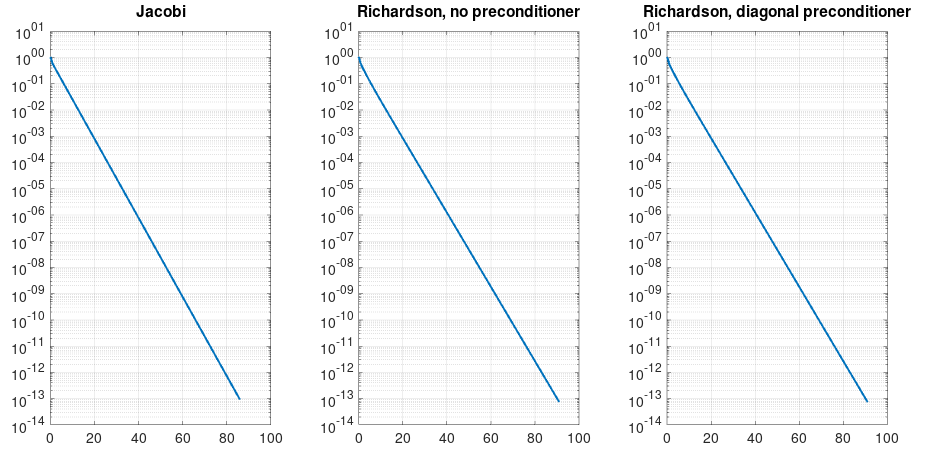
\includegraphics[width=\textwidth]{figure1.png}
\end{center}
We notice the plots for Richardson's method with or without
preconditioner are identical, this makes sense, since the diagonal
of $A$ is just $2I_3$ and so the $\alpha$ we used reverts the
change made by the preconditioner. We notice Jacobi's method
performs silghtly better, so the $\alpha$ used was not optimal.

Below follow the plots for the matrix \texttt{matr} provided in the
exercise.
\begin{center}
	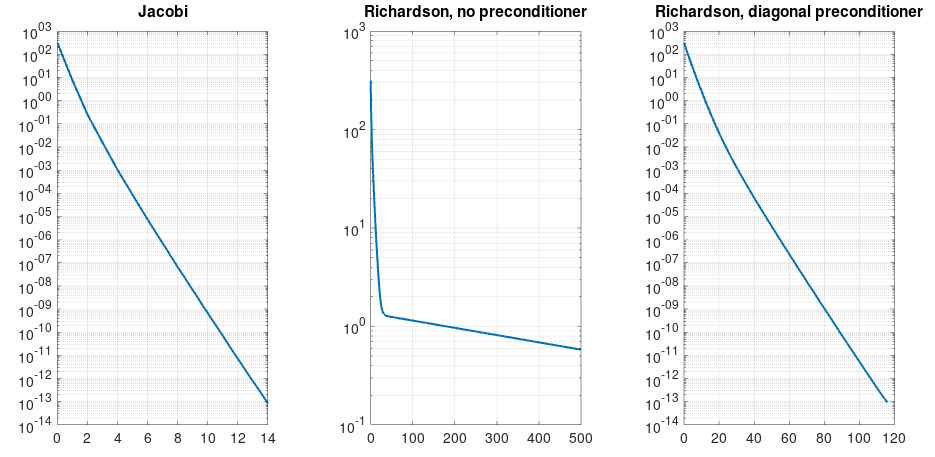
\includegraphics[width=\textwidth]{figure2.png}
\end{center}
We notice Jacobi's method greatly outperforms both Richardson's
method with and without preconditioner.
Richardson's method without preconditioner converges very slowly,
which is probably due to a very high condition number (as
the matrix is very large, Matlab cannot compute the condition
number, so it's just a guess). For Richardson's method with
diagonal preconditioner, this is clearly due to a bad choice of
$\alpha$, as Jacobi's method is just a special case of
Richardson's method with diagonal preconditioner.

\end{document}
